%    Noveno Capítulo: subtipificado.
%    Ejercicios por Barón L. Miguel.
%    Teoría por Javier Enríquez Mendoza.
%    Empezado el 19/7/23
%    Concluido el 3/8/23

%Gatito lambda
\begin{figure}[htbp]
    \centerline{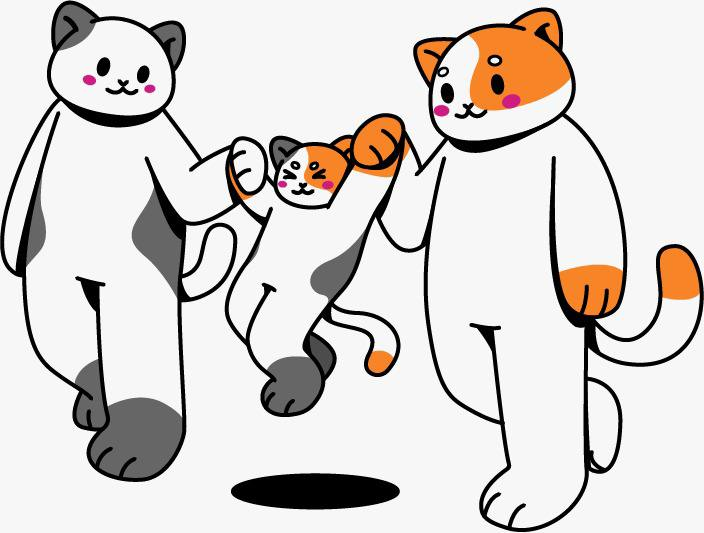
\includegraphics[scale=.5]{assets/10_gatitos_familia.jpg}}
\end{figure}

En este capítulo vamos a revisar el último paradigma de programación que estudiaremos en este manual: La orientación a objetos y sus características más importantes como la herencia y los subtipos.\\\\
La introducción del paradigma de la orientación a objetos presenta una ventaja al momento de reutilizar código que ya hemos definido anteriormente y que durante los últimos años supuso una revolución en la forma en la que se escriben y desarrollan los programas que corren en nuestros teléfonos y computadoras personales.\\\\
Lenguajes como \textsf{Java},  \textsf{Python}, \textsf{Ruby}, \textsf{Golang}, \textsf{Swift}, \textsf{C\#} entre muchos otros implementan la herencia, en donde métodos, constructores y variables de la clase padre puede ser reutilizadas por otra clase hija.\\\\
Más aún, en este tipo de lenguajes la flexibilidad no solo se extiende a hacer uso de código previamente definido y heredado si no que se puede extender y sobrecargar sobre lo ya existente, proporcionando una mecanismo modular para desarrollar software y evitar la re definición de clases, métodos y variables. 

\subsubsection{Objetivo}
El objetivo de este capítulo es proporcionar una definición de los conceptos principales de la orientación objetos y su aplicación a la herencia y el subtipificado en el paradigma procedimental para las diferentes categorías definidas en la sintaxis de \textsf{TinyC}.

\subsubsection{Planteamiento}
En este capítulo se presentan las definiciones principales del paradigma de la orientación a objetos como clase, objeto y subtipo, así como las reglas que nos permiten inferir el tipo de una expresión.\\\\
Finalmente se concluye el capítulo introduciendo el concepto de $casting$ (en español conversión) junto con los juicios que nos permiten transformar el tipo de una expresión. 

\section{Orientación a objetos}
La orientación a objetos tiene como fundamento la abstracción de los elementos mas importantes de las entidades que se desean modelar en la computadora, su identidad, su comportamiento, relaciones, etc. Para este propósito se utiliza una abstracción conocida como clase. 

\begin{definition}[Definición para clases]\footnote{Definición formulada de \hyperlink{128}{[128]} y \hyperlink{133}{[133]} }\\
    Una clase es una abstracción de una entidad, elemento u objeto que define sus características más importantes como el nombre, los atributos, variables y métodos que describen su comportamiento.
\end{definition}

\bigskip

\begin{definition}[Definición de objeto]\footnote{Definición formulada de \hyperlink{128}{[128]} y \hyperlink{133}{[133]} }\\
    Un objeto es una instancia de una clase.
\end{definition}

\bigskip

Las características que se comparten entre los lenguajes que implementan este paradigma incluyen\footnote{Definición formulada de \hyperlink{133}{[133]}} 
\begin{itemize}
    \item \textbf{Herencia:}
	 Permite la definición de una clase original dejando que esta sea extendida o sobrecargada por las clases que heredan de ella, constituyendo un mecanismo para reutilizar código previamente escrito y adaptarlo al contexto particular donde se desean instanciar los objetos.\\

    \item \textbf{Encapsulamiento de datos:} Comprende la seguridad de la información contenida en las variables y métodos de una clase. Permitiendo que solo el objeto mismo sea el encargado de alterar la información contenida en él, proporcionando seguridad y consistencia.\\

    \item  \textbf{Polimorfismo:} Esta característica permite que un objeto que ha heredado de una clase pueda ser identificado por cualquiera de los tipos que posea la cadena de herencia, pudiendo este ser su mismo tipo, o cualquiera de los tipos de la clase o clases padres.\\\\
Esta característica es diferente al polimorfismo que se estudia en lenguajes funcionales, donde por ejemplo la función \textsf{id} :: $a$ $\rightarrow$ $a$ puede ser tipificada con el tipo del argumento que la aplique.\\\\
 En Java el polimorfismo se aplica en la sobrecarga de métodos para reutilizar los definidos por la clase que se está extendiendo.\\

    \item \textbf{Representaciones múltiples:} Permite que dos objetos de una misma clase puedan presentar comportamiento distinto pues este puede cambiar según el estado que posea cada uno.\\

    \item \textbf{Recursión abierta:} Un objeto es capaz de invocarse a si mismo dentro de la definición de los métodos de su propia clase, utilizando las palabras reservadas como \textsf{self} o \textsf{this}.
\end{itemize}


\section{Subtipos}

Los sistemas de tipos que hemos estudiado hasta este momento son restrictivos en el sentido de que muchas operaciones que parecerían intuitivas al desarrollar un programa no serían aceptadas por dicho sistema.
Particularmente operaciones como la suma (+) entre los tipos $Int$ y $Float$ por ejemplo.\\\\
Necesitamos ''relajar'' este sistema para tener mas flexibilidad sobre este tipo de casos. En particular necesitamos construir la relación de subtipificado; A $\leq$ B que simboliza: ''A es subtipo de B''.

\begin{definition}[Relación de subtipificado]\footnote{Definición formulada de \hyperlink{130}{[130]}, \hyperlink{131}{[131]} y \hyperlink{132}{[132]} } \\

        \begin{description}
        	\item[Reflexividad]
        	$$\inference{}{A \leq A}$$
        	\item[Transitividad]
        	$$\inference{A\leq B & B \leq C}{A \leq C}$$
        	\item[Subsunción]
        	$$\inference{\Gamma \vdash e:A & A \leq B}{\Gamma\vdash e:B}$$
        	Esta propiedad expresa que si una expresión tiene tipo  A$\,$ y A$\,$ es subtipo de B$\,$ entonces puede usarse en cualquier contexto en donde sea necesaria una expresión de tipo B.
        \end{description}
    \end{definition}
    
 \begin{exercise} Para este ejemplo consideremos la expresión:
    
    $$ 5.5 + 2$$
    Donde podemos observar que $5.5:Float$ y $2:Int$, suponemos entonces que los tipos $Float$ e $Int$ están relacionados bajo subtipificado como 
    $$Int\ \leq\ Float$$
    por lo que la derivación de tipos de la expresión anterior queda como sigue:
    \[
    	\inference
    	{
    		\inference{}{\varnothing\vdash 5.5: Float}&
    		\inference
    		{
    			\inference{}{\varnothing\vdash 2:Int}&
    			Int \leq Float
    		}
    		{\varnothing\vdash 2:Float}
    	}
    	{\varnothing\vdash 5.5+2:Float}
    \]
    
    Gracias a la propiedad de subsunción podemos reemplazar $Int$ por $Float$ en la derivación de los tipos conservando la propiedad de ser una expresión válida\footnote{Ejemplo extraído de \hyperlink{5}{[5]}  }.
\end{exercise}

\bigskip

La relación de subtipificado puede ser aplicada a partir de dos interpretaciones diferentes\footnote{Definición formulada de \hyperlink{5}{[5]}, \hyperlink{12}{[12]} }:
\begin{itemize}

\item \textbf{Interpretación por subconjuntos:} sí A $\leq$ B entonces toda expresión de tipo A también es una expresión de tipo B pues A está contenido en B.\\
\item \textbf{Interpretación por coerción:} entendemos coerción como la acción de ejercer presión sobre un objeto para forzar su conducta. Esta acción aplicada al contexto de software nos permite modelar el siguiente comportamiento: sí $s\ :\ A$ y $A\ \leq \ B$ entonces $s$ se puede convertir de forma única a una expresión de tipo $B$, es decir forzamos el cambio de tipo mediante una conversión explícita.\\\\
    En el ejemplo anterior teníamos 2 : $Int$ el cuál fue coercido a 2.0 : $Float$.\\

\end{itemize}

    
\subsection{Subtipificado de tipos primitivos}
    Las reglas para definir la relación de subtipificado entre los tipos primitivos proporcionados en la definición de los lenguajes de programación, constituyen los axiomas de dicho sistema y con ellos se pude derivar el resto de las reglas utilizando las propiedades de subsunción y transitividad.\\\\
    Para ilustrar este punto se agrega el tipo $Float$ junto con los axiomas:
    
\begin{definition}[Relación de subtipificado para $Nat,\ Int\ y\ Float$]\footnote{Definición formulada de \hyperlink{130}{[130]}, \hyperlink{131}{[131]} y \hyperlink{132}{[132]} }
    \[
    	\begin{array}{ccc}
    	\inference{}{Nat \leq Int}&\qquad\qquad&\inference{}{Int \leq Float}
    	\end{array}
    \]
\end{definition}

\subsection{Subtipificado de funciones}

    Definamos el siguiente tipo para una función $f$ como $f:Int \to Int$, entonces se tiene que $f\,n : Int$,  $\forall \ n:Int$. Aplicando la regla de subsunción obtenemos $f\,n: Float$, y por consiguiente:
    $$Int \to Int \leq Int \to Float$$ es una derivación de tipo válida.
    Es decir la relación de subtipificado original se preserva en el codominio de la función. En tal caso se dice que esta posición es covariante.
    
    Por otro lado si definimos el tipo de nuestra función como $f: Float \to Int$. Tenemos que como todas las expresiones $e:Int$ son también de tipo $Float$  podemos utilizar la relación de subtipificado en sentido opuesto para restringir el dominio (de forma inversa a como se usó en el caso anterior), así podemos introducir elementos de tipo $Int$ en el dominio de $f$. Por lo que se cumple la siguiente relación de subtipificado:
    $$Float \to Int \leq Int \to Int$$ 
    Es decir, la relación de subtipos original $Int \leq Float$ usada en la primera derivación se invierte para este caso, decimos entonces que este argumento es contravariante.
    
    Finalmente, usando la propiedad de transitividad tenemos la siguiente relación de subtipificado
    $$Float \to Int \leq Int \to Int \leq Int \to Float $$
    De esta forma podemos definir la regla de subtipificado para el caso general de los tipos función como sigue\footnote{fragmento extraído de \hyperlink{5}{[5]}  }.

\begin{definition}[Definición para subtipificación de funciones]\footnote{Definición formulada de \hyperlink{5}{[5]}, \hyperlink{12}{[12]}, \hyperlink{131}{[131]} y \hyperlink{132}{[132]} }\\
    $$\inference{T_1 \leq S_1 & S_2 \leq T_2}{S_1 \to S_2 \leq T_1 \to T_2}$$
\end{definition}
    
\subsection{Subtipificado para suma y producto}
    Para esta aplicación la relación de subtipificado se comporta como contravariante, es decir la dirección de la relación se preserva como es de esperar, de tal forma que se introducen las siguientes reglas al sistema de tipos.
    
\begin{definition}[Reglas para subtipificar expresiones aritméticas]\footnote{Definición formulada de \hyperlink{5}{[5]}, \hyperlink{12}{[12]}, \hyperlink{131}{[131]} y \hyperlink{132}{[132]} }\\
    \[
    	\begin{array}{ccc}
    		\inference{S_1 \leq T_1 & S_2 \leq T_2}{ S_1 + S_2 \leq T_1 + T_2}&\qquad\qquad\qquad&
    		\inference{ S_1 \leq T_1 & S_2 \leq T_2}{S_1 \times S_2 \leq T_1 \times T_2}
    	\end{array}
    \]
\end{definition}
    
\subsection{Subtipificado para registros}

    Los registros, como hemos estudiado en secciones anteriores, son la generalización de una tupla permitiendo extender el concepto para $n$ elementos. Asociadas a estos existen las proyecciones para recuperar el n-ésimo elemento contenido en esta estructura.

    Veremos brevemente las características asociadas al tipo de los registros una vez se introduce la relación de subtipificado.
 
\begin{definition} [Definición de la relación de subtipificado aplicado a los tipos registros]\footnote{Definición formulada de \hyperlink{5}{[5]}, \hyperlink{12}{[12]}, \hyperlink{131}{[131]} y \hyperlink{132}{[132]} }\\
    \begin{description} 
    	\item \textbf{Amplitud} Dados dos registros A y B donde A posee una cantidad mayor de elementos que B, decimos que el tipo del registro A es subtipo del registro B representado de la siguiente forma:
    
    	$$\inference{}{(l_1:T_1,\dots,l_{n+k}:T_{n+k})\leq(l_1:T_1,\dots,l_{n}:T_{n})}$$ \\
    
    	\item \textbf{Profundidad} Esta propiedad es la aplicación de la covarianza de la relación de subtipificado, aplicándose a cada uno de los campos contenidos en el registro:
    
    	$$\inference{T_1 \leq S_1 & \cdots & T_n \leq S_n}{(l_1:T_1,\dots,l_{n}:T_{n})\leq(l_1:S_1,\dots,l_{n}:S_{n})}$$\\
    
    	\item \textbf{Permutación} El orden de los campos de un valor de tipo registro no importa.
    
    	$$\inference{(s_1:S_1,\dots,s_{n}:S_{n})\mbox{ permutación de }(l_1:T_1,\dots,l_{n}:T_{n})}{(s_1:S_1,\dots,s_{n}:S_{n})\leq(l_1:T_1,\dots,l_{n}:T_{n})}$$

    \end{description} 
\end{definition}

\subsection{Elementos máximos}
 
        En nuestra implementación para el sistema de tipos es importante contar con un elemento máximo, en donde todo elemento distinto al elemento máximo es subtipo de este. Aquí  introducimos $Top$ que cumple exactamente con esta característica representada de la siguiente forma:

\begin{definition}[Definición del elemento \textit{Top} para el sistema de subtipificado]\footnote{Definición formulada de \hyperlink{5}{[5]}, \hyperlink{12}{[12]}}
    
        $$ \inference{}{T \leq Top}$$
    
\end{definition}
        La idea detrás de $Top$, es que a este tipo pertenecen todos aquellos programas que están correctamente tipificados. En Java a este tipo se le conoce como $Object$.\\
        
        El contrario, es un tipo que es subtipo de todos y se conoce como $Bot$, este es inhabitado, ninguna expresión debe de existir dentro del mismo.
        Este tipo ayuda a expresar aquellos programas que no deben de regresar ningún valor, similar a la forma en la que se utiliza el tipo $void$ en Java.\\\\
        La descripción anteriormente dada para $Bot$ se representa de la siguiente forma:

\begin{definition}[Definición del elemento \textit{Bot} para el sistema de subtipificado]\footnote{Definición formulada de \hyperlink{5}{[5]}, \hyperlink{12}{[12]}}
        $$ \inference{}{Bot \leq T}$$
\end{definition}

\section{Conversión de tipos}

    En lenguajes de programación como Java hemos hecho uso de este mecanismo para cambiar el tipo de un dato o variable por otro. \\\\
    Similar al ejemplo que tenemos para pasar de 2 :\textit{ Int} a 2.0 :\textit{ Float}.
    La relación de subtipificado nos provee la regla de subsunción. Sin embargo definiremos el mecanismo para ambos sentidos de la relación conocidos como conversión ascendente (\textit{Upcasting}) y conversión descendente (\textit{Downcasting}).\\

    \subsection{Conversión ascendente \it (Upcasting)}
        En este tipo de casting (también conocido como ''casting hacia arriba'') el objetivo es que al tipificar un término, a este se le atribuye un supertipo esperado. \\\\
	  De esta forma  para los subtipos donde $T \leq R$ entonces usando subsunción podemos concluir que $\Gamma \vdash \< R \> \,e:R$, en donde $\<R\>$ es la notación para el {\it casting} explícito, representado como:
	\begin{definition}[Definición para Conversión ascendente]\footnote{Definición formulada de \hyperlink{5}{[5]}, \hyperlink{12}{[12]}, \hyperlink{131}{[131]} y \hyperlink{132}{[132]} }:
        $$\inference{\Gamma\vdash e:T & T \leq R}{\Gamma\vdash\<R\>\,e:R}$$
	\end{definition}
    \subsection{Conversión descendente \it (Downcasting)}
        En este tipo de casting (también conocido como ''casting hacía abajo'') la asignación de tipos es arbitraria, la relación de subtipificado no necesariamente se tiene que cumplir.\\\\
        Esto supone una amenaza a la consistencia de tipos en el programa que se escribe con esta instrucción, el lenguaje está forzado a aceptar el \textit{downcasting} en tiempo de compilación pero en tiempo de ejecución un futuro conjunto de verificaciones deben de ser ejecutados para corroborar que el tipo asignado no supone un error. Esta regla se representa de la siguiente manera: 

	\begin{definition}[Definición para conversión  descendente]\footnote{Definición formulada de \hyperlink{5}{[5]}, \hyperlink{12}{[12]}, \hyperlink{131}{[131]} y \hyperlink{132}{[132]} }:
        $$\inference{\Gamma\vdash e:T}{\Gamma\vdash\< R\>\,e: R}$$
	\end{definition}

\section{Ejercicios para el lector}


    \begin{exercise}
        Dada la siguiente expresión, utiliza las reglas de tipificado para suma y producto para derivar el tipo de la misma.
        $$ 4.0\ - \ 1\ < \ 3.0\ : \ \textit{Float}$$
    \end{exercise}

    \bigskip

    \begin{exercise}
        Dada la siguiente expresión, utiliza las reglas de tipificado para suma y producto para derivar el tipo de la misma.
        $$ 3\ +\ 3.0 \ +\ 4\ - \ 4\ : \ \textit{Float}$$
    \end{exercise}
    \bigskip

    \begin{exercise}
        Dada la siguiente expresión, utiliza las reglas de tipificado para el operador \textit{if} y deriva el tipo de la misma.
        $$\textsf{if } 7\ *\ 0.0 < 0 \textsf{ then } 1 \textsf{ else } 0 : \ \textit{Float}$$
    \end{exercise}
    \bigskip

    %\begin{exercise}
      %  Dada la siguiente expresión, utiliza las reglas de tipificado para el operador \textit{while} y deriva el tipo de la misma.
        %$$ \textsf{Int}\ i\ =\ 0;\ \textsf{while}(i < 10)\{i + 1;\}\ \textsf{return } i;\ :\ Float$$
    %\end{exercise}
   % \bigskip

    \begin{exercise}
        Dada la siguiente expresión, utiliza las reglas de tipificado para el operador \textsf{fun} y deriva el tipo de la misma.
        $$ \textsf{fun}(x:\textsf{Int} \rightarrow \ x + 1\ ) : \textit{Int}  \rightarrow \textit{Float} $$
    \end{exercise}

    \bigskip

    \begin{exercise}
        Utiliza la regla de \textit{Upcasting} para obtener el tipo de la siguiente expresión basado en las reglas para tipos primitivos.
        $$ \textsf{fun}(x:\textsf{Int} \rightarrow \textsf{if}\ x < 0\ \textsf{then}\ x - 1.0 \ \textsf{else}\ x ) : \textit{Int}  \rightarrow \textit{Int} $$
    \end{exercise}

    \bigskip

    \begin{exercise}
        Utiliza las reglas de elementos máximos para obtener la derivación del tipificado para la siguiente expresión.
        Si no es posible argumenta por qué.
        $$\textsf{fun}(x:\textsf{Int} \rightarrow \textsf{if}\ x \leq 0\ \textsf{then}\ x - 1.0 \ \textsf{else}\ x   ) : \textit{Bot} $$
    \end{exercise}
	
	\bigskip

    \begin{exercise}
        Utiliza las reglas de elementos máximos para obtener la derivación del tipificado para la siguiente expresión.
	  Si no es posible argumenta por qué.
        $$ \textsf{fun}(x:\textsf{Int} \rightarrow \textsf{if}\ x \leq 0\ \textsf{then}\ x - 1.0 \ \textsf{else}\ x) : \textit{Top} $$
    \end{exercise}
 